
\chapter{Oscillazioni smorzate e forzate}


\section{Introduzione}

Oggetto di questa ricerca è lo studio delle oscillazioni smorzate e forzate di un pendolo. Studiando il variare delle oscillazioni al variare della frequenza operativa della forzante, si studierà il fenomeno della risonanza.

\subsection{Strumenti}
\begin{center}
\begin{tabular}{l|l}
\midrule
Strumento & Precisione\\
\midrule
Calibro & $\pm 0.05$ mm\\ 
Sensore di rotazione & $\pm 0.00157$ rad\\ 
Alimentatore & $\pm 0.01$ V\\ 
\midrule 
\end{tabular}
\end{center}
L'attrezzatura utilizza è costituita da un disco metallico fissato ad una puleggia. La puleggia è messa in oscillazione da un filo alle cui estremità vi sono un oscillatore  elettromeccanico, che agisce come forzante, e un sistema di due molle. Al disco è possibile avvicinare e allontanare un magnete, che ha la funzione di smorzare il moto.

\subsection{Oscillazioni libere}

Si pone in oscillazione il disco, con il magnete  posizionato lontano e l'oscillatore elettromeccanico spento. Un sensore di posizione misura lo spostamento angolare; il sensore è collegato ad un computer, ed il programma DataStudio traccia in tempo reale il grafico dello spostamento angolare in funzione del tempo. Si interpolano dunque i dati con una funzione sinusoidale per determinare il periodo e la pulsazione delle oscillazioni e si ricava: $$T=1.47\pm0.02\ s \hspace{1cm} \omega=4.272\ rad/s$$ L'errore riportato è quello che il programma stesso attribuisce alla rilevazione, ed è determinato dalla precisione degli strumenti di rilevamento e dall'interpolazione dei dati.

\subsection{Oscillazioni smorzate}

Si avvicina il magnete al disco metallico. Il moto oscillatorio risulterà così smorzato per effetto delle correnti di Focault.
I dati raccolti dal sensore sono stati interpolati con la funzione
$$ \theta (t) = A_0 e^{- \gamma t} \sin(wt+\phi)+\theta_0 $$
al fine di determinare i parametri liberi; i valori ottenuti sono riportati di seguito in tabella.\\

$$T=1.45\ s$$

\begin{center}
\begin{tabular}{l|l|l}
\midrule
Parametri & Valore ricavato & $ \pm \sigma$ \\
\midrule
$A_0$ & 3.08 rad & 0.020\\
$\gamma$ & 0.197 $m^4/kg$& 0.0019\\
$\omega$ & -4.27 rad/s& 0.0019\\
$\phi$ & 1.93 rad & 0.0069 \\
$\theta_0$ & -1.53 rad& 0.0019 \\
\midrule
\end{tabular}
\end{center}

A questo punto, noti $\omega$ e $\gamma$, è possibile calcolare $ \omega_0 $, cioè la pulsazione per le oscillazioni libere, tramite l'equazione:
\begin{equation}\label{eq:omega}
\omega = \sqrt{\omega_0^2 - \gamma^2}
\end{equation} da cui:
$$\omega_0 = 4.275\ rad/s$$

Confrontandolo con il valore che avevamo ricavato interpolando direttamente il grafico delle oscillazioni libere si nota che i due non coincidono, ma che quello misurato dal periodo delle oscillazioni libere è minore di quello ricavato dalla formula: infatti, essendo un sistema reale, tra le sue parti sono presenti degli attriti che smorzano le oscillazioni.

\section{Oscillazioni smorzate-forzate}

Mantenendo il magnete vicino al disco, si mette in azione l'oscillatore elettromeccanico, che fornisce una componente forzante. Variando il voltaggio dell'alimentatore,  la frequenza di rotazione dell'oscillatore cambia: cerchiamo la frequenza di risonanza del sistema.
Poiché il periodo dell'oscillatore armonico coincide con quello della forzante (prima di raccogliere i dati si attende che il sistema si sia stabilizzato), possiamo leggere direttamente il periodo dal valore restituito dalla fotocellula.
Dopodiché abbiamo interpolato questi dati con il programma DataStudio, secondo la funzione
\begin{equation} \label{A}
A(\omega) = \frac{M_0}{\sqrt{ ({\omega_0}^2-\omega^2)^2 + 4\gamma^2\omega^2}}
\end{equation}

ed abbiamo ricavato così i valori corrispondenti ai parametri liberi $M_0$, $\gamma$ e $\omega_0$. 

Tale procedura è stata ripetuta spostando il magnete a distanze differenti dal disco.
\\
Di seguito sono riportati i dati raccolti e i rispettivi grafici. Di fianco alle tabelle si trovano i parametri ricavati dall'interpolazione con una sinusoidale, mentre sotto i grafici i valori ottenuti dall'interpolazione con la funzione \ref{A}. Tra la tabella e il grafico si trova invece il valore di $\omega_0$ ottenuto dalla \ref{eq:omega}.

\subsubsection{4.80mm}

\begin{center}
\begin{tabular}{c c}
\begin{tabular}{c | c | c}
\textbf{Ampiezza ($rad$)} & \textbf{Periodo ($s$)} & \textbf{Pulsazione ($rad/s$)}\\
\midrule
0.89 & 5.45 & 1.15\\
0.94 & 4.78 & 1.31\\
1.05 & 3.57 & 1.75\\
1.09 & 3.19 & 1.97\\
1.30 & 2.46 & 2.55\\
1.30 & 2.59 & 2.42\\
1.84 & 2.06 & 3.05\\
1.91 & 1.90 & 3.31\\
3.42 & 1.70 & 3.69\\
6.35 & 1.59 & 3.95\\
1.19 & 1.14 & 5.51\\
\end{tabular}

& 
\begin{tabular}{c}
$M_0=15.13\pm0.27$\\
\\
$\omega_0=4.25\pm0.01\ rad/s$\\
\end{tabular} 

\end{tabular}

\end{center}
 
\begin{center}

\includegraphics[scale=0.5]{"../grafici/Magnetea48mm"}

$$ \omega_0 = 4.25\ rad/s $$
$$ \gamma = 0.193\ s^{-1}$$
$$ M_0 = 15.3\ s$$


\end{center}
 
 
\subsubsection{2.80mm}

\begin{center}

\begin{tabular}{c c}

\begin{tabular}{c | c | c}
\textbf{Ampiezza} ($rad$) & \textbf{Periodo} ($s$) & \textbf{Pulsazione} ($rad/s$)\\
\midrule
1.68 & 2.00 & 3.14\\
2.95 & 1.63 & 3.85\\
3.22 & 1.44 & 4.36\\
2.17 & 1.30 & 4.83\\
1.20 & 1.15 & 5.46\\
1.67 & 1.24 & 5.06\\
0.99 & 1.10 & 5.71\\
0.68 & 0.98 & 6.40\\
0.51 & 0.89 & 7.06\\
0.26 & 0.74 & 8.49\\
\end{tabular}

& \hspace{1cm}

\begin{tabular}{c}
$A_0 = 3.4 \pm 0.020\ rad$\\
\\
$\gamma =  0.636 \pm 0.0057\ m^4/kg $\\
\\
$\omega = -4.25  \pm 0.0064\ rad/s $\\
\\
$\phi =  2.38 \pm 0.0076\ rad $ \\
\\
$\theta_0 = -0.57 \pm 0.0038\ rad $\\

\end{tabular}

\end{tabular}

\end{center}

$$\omega_{0} = 4.297\ rad/s$$
\begin{center}
\includegraphics[scale=0.5]{"../grafici/Magnetea28mm"}

$$ \omega_0 = 4.26\ rad/s $$
$$ \gamma = 0.543\ s^{-1} $$
$$ M_0 = 15.6\ s$$

\end{center}


\subsubsection{1.00mm}

\begin{center}

\begin{tabular}{c c}

\begin{tabular}{c | c | c}

\textbf{Ampiezza} ($rad$) & \textbf{Periodo} ($s$) & \textbf{Pulsazione} ($rad/s$)\\
\midrule
1.33 & 2.01 & 3.12\\
1.42 & 1.85 & 3.39\\
1.45 & 1.67 & 3.76\\
1.18 & 1.31 & 4.79\\
1.31 & 1.39 & 4.52\\
1.47 & 1.54 & 4.07\\
0.76 & 1.09 & 5.76\\
0.88 & 1.19 & 5.28\\
1.01 & 1.22 & 5.15\\
0.49 & 0.93 & 6.75\\
0.65 & 1.03 & 6.10\\
0.39 & 0.85 & 7.39\\

\end{tabular}

& \hspace{1cm}

\begin{tabular}{l}

$A_0 = 18600 \pm 1300\ rad$ \\
\\
$\gamma= 1.50 \pm 0.0011\ m^4/kg$\\
\\
$\omega = 4.02 \pm 0.0077\ rad/s$\\
\\
$\phi =  26.3 \pm 0.0046 \ rad/s$ \\
\\
$\theta_0 = 0.055 \pm 0.0016\ rad$ \\

\end{tabular}

\end{tabular}

\end{center}


$$\omega_{0} = 4.291\ rad/s $$

\includegraphics[scale=0.75]{"../grafici/Magnetea10mm"}


$$ \omega_0 = 4.37\ rad/s $$
$$ \gamma = 1.40 \pm 0.14\ s^{-1}$$
$$ M_0 = 17.1 \pm 1.4\ s$$


\section{Risonanza}
\section{Conclusioni}
L'esperimento è riuscito un sacco.

\section{Fenomeno}
Sovvrapponendo le curve trovate in precedenza, possiamo apprezzare un grafico nel quale si mette in evidenza la risonanza. 
Verifichiamo anche la condizione di risonanza Con l'approssimarsi di $\gamma $ a zero, il valore dell'ampiezza tende a $\infty$.









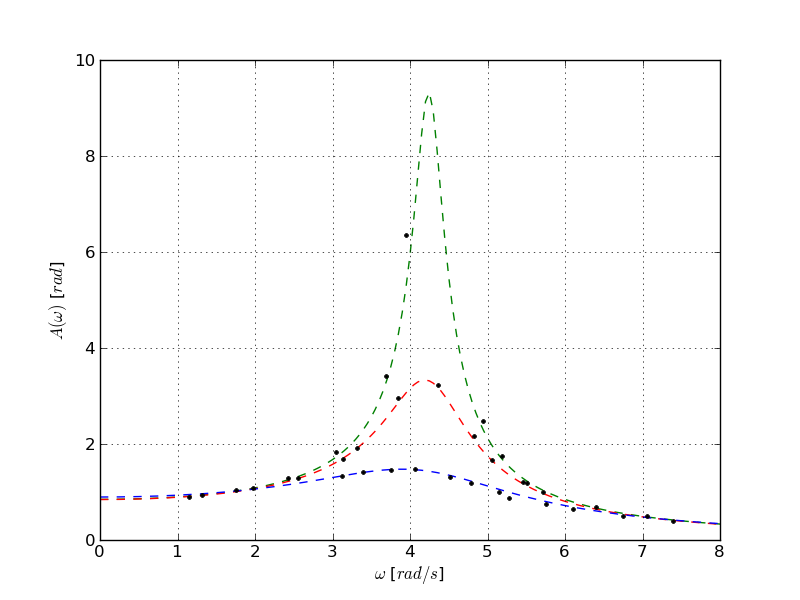
\includegraphics[scale=0.9]{../grafici/risonanza.png}
